%\title{Experiential Learning Spring Symposium Presentation}
\documentclass[10pt]{beamer}

\usetheme[progressbar=frametitle]{metropolis}
\usepackage{appendixnumberbeamer}

\usepackage[compatibility=false]{caption}
\usepackage{subcaption}
\usepackage{csquotes}
\usepackage{booktabs}
\usepackage{hyperref}
\usepackage[scale=2]{ccicons}
\usepackage{tikz}
\usetikzlibrary{positioning}
\usetikzlibrary{3d}

\usepackage{multimedia}
\usepackage{media9}

\usepackage{pgfplots}
\usepgfplotslibrary{dateplot}

\usepackage{xspace}
\newcommand{\themename}{\textbf{\textsc{metropolis}}\xspace}

\usepackage{pdfpages}


\title{COMAP Mathematical \\ Competition in Modeling 2017}
\subtitle{Experiential Learning Spring Symposium}
\date{April 27th, 2017}
\author{\texorpdfstring{Matthew Moreno \newline\url{mamoreno@pugetsound.edu}}{Matthew Moreno}}
\titlegraphic{\hfill
\includegraphics[height=2cm]{img/UofPS_stacked_maroonRGB_PNG.png}}


\definecolor{h1}{HTML}{d19a66}
\definecolor{h2}{HTML}{36a8b8}

\begin{document}

\maketitle

{
\setbeamercolor{background canvas}{bg=}
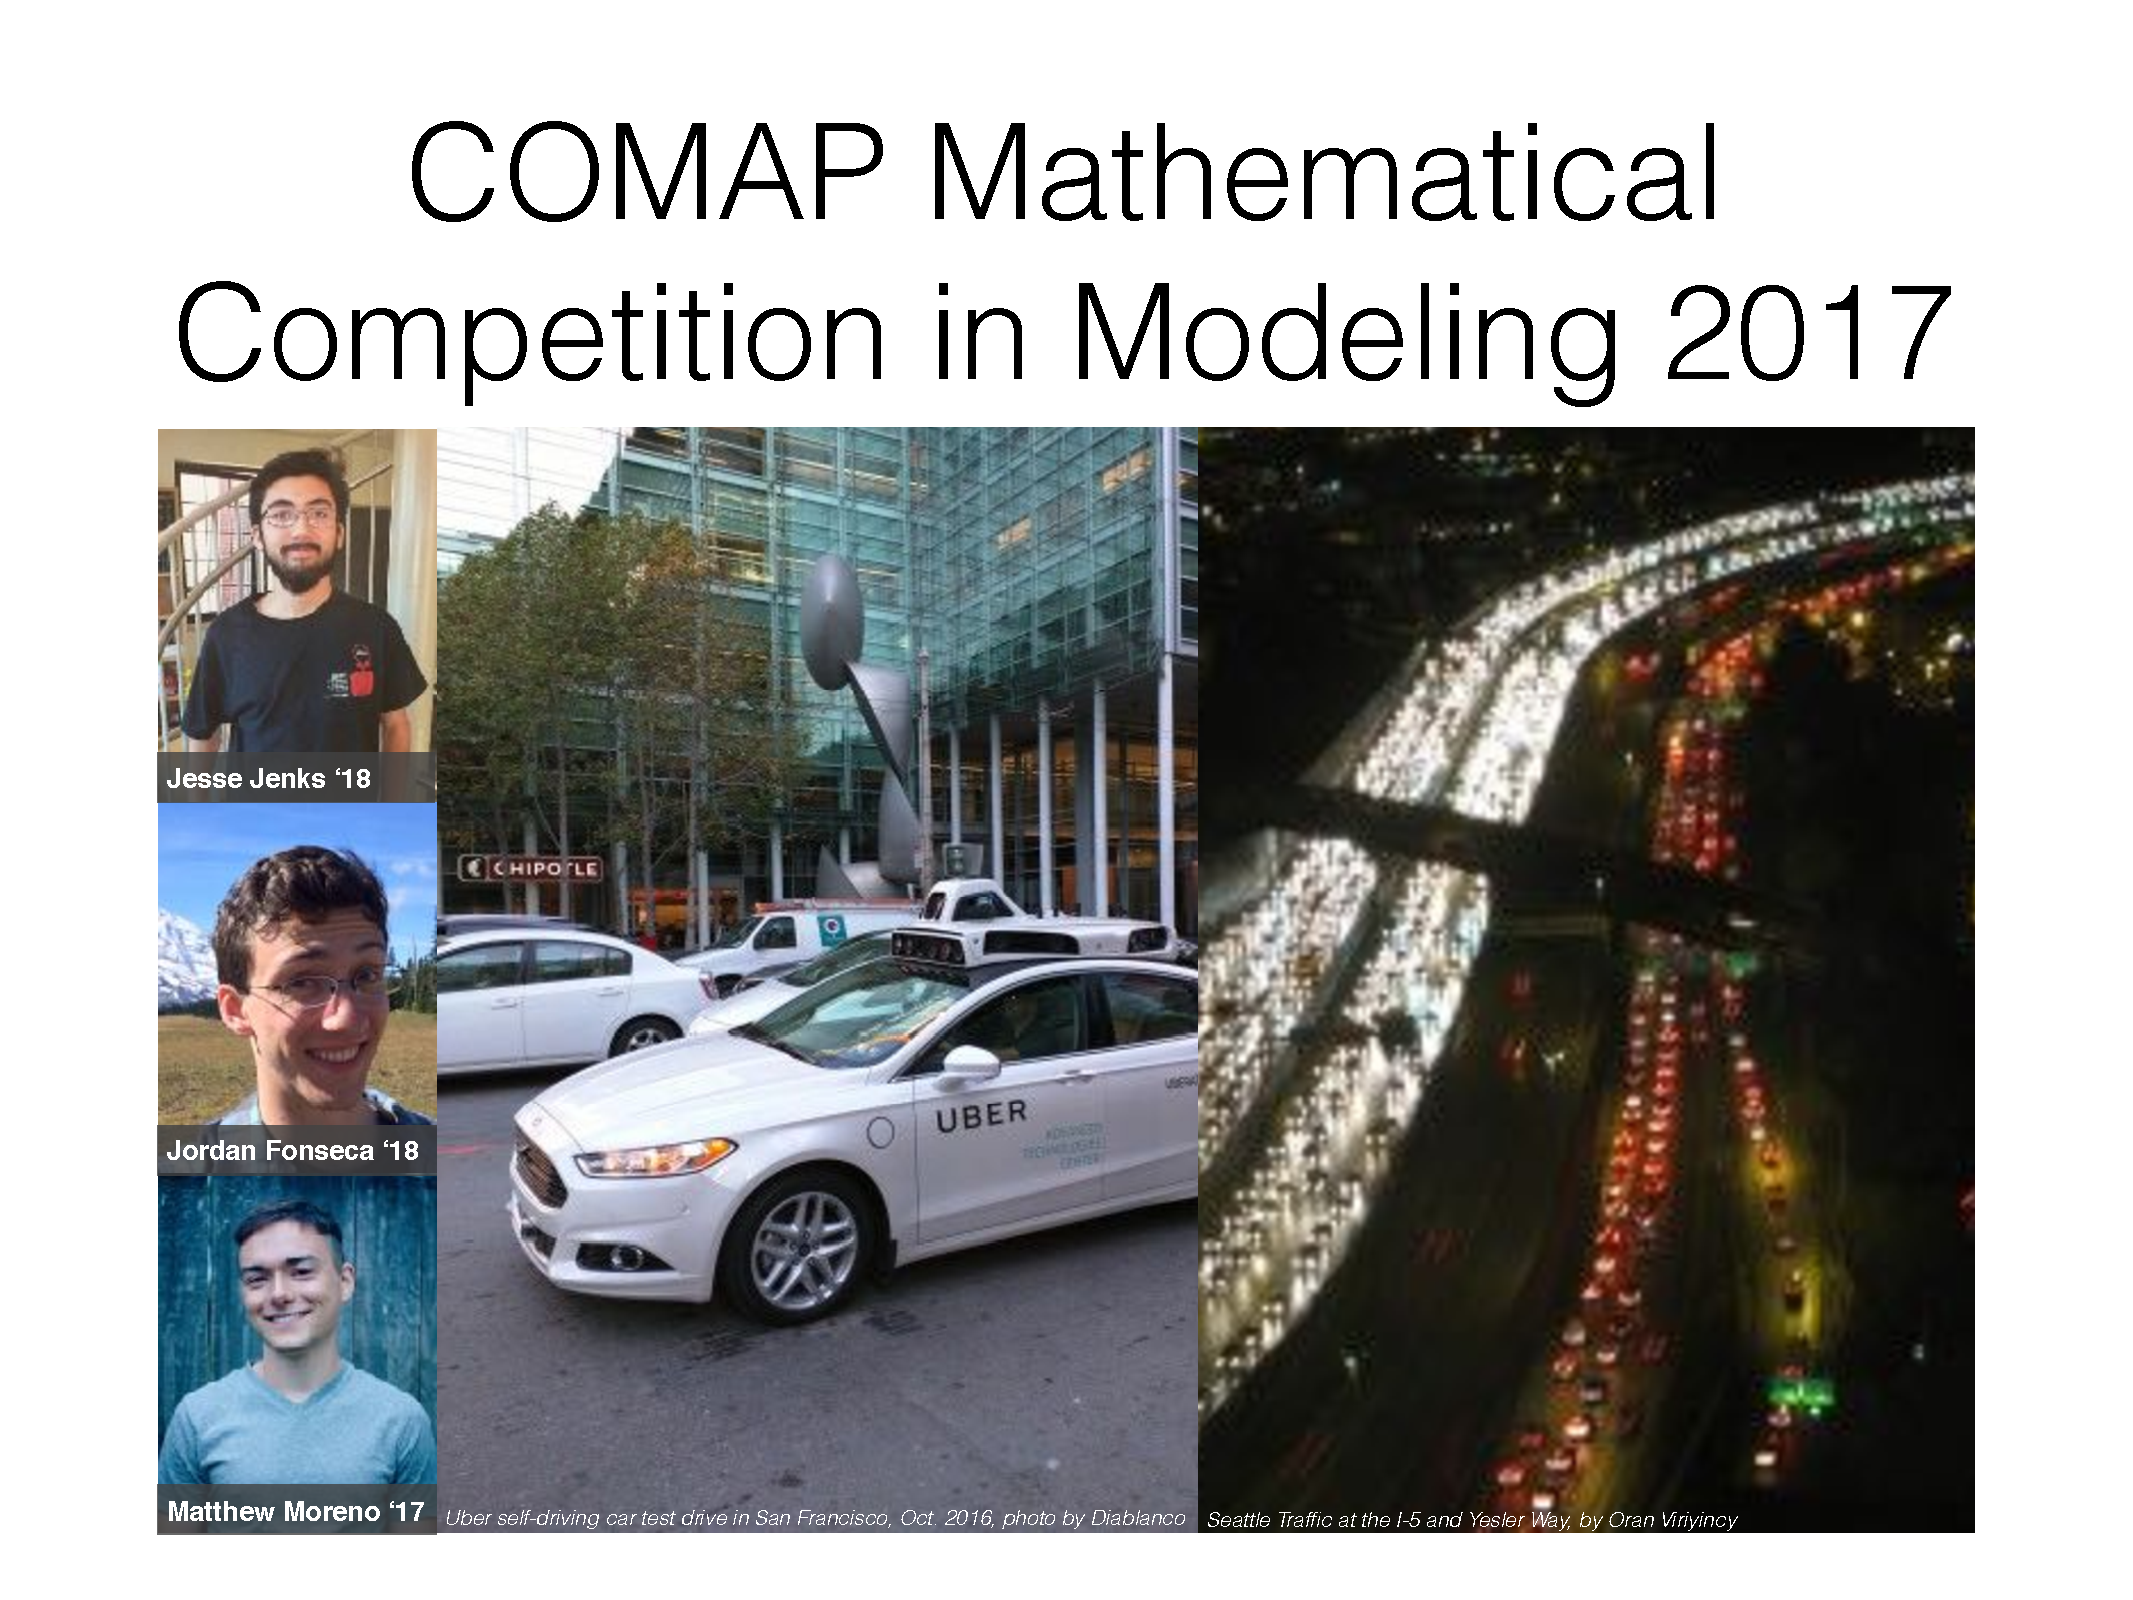
\includepdf[pages={1}]{img/experiential_learning_symposium_2017.pdf}
}


\appendix

\begin{frame}{Acknowledgements}

\begin{itemize}
\item University of Puget Sound Mathematics \& Computer Science Department for sponsoring our team
\item Professor Spivey, MCM advisor and coordinator
\end{itemize}
	\vspace{-1ex}
	\begin{center}{
    
\includegraphics[width= 0.3\textwidth]{img/UofPS_stacked_maroonRGB_PNG}}
    \end{center}

\end{frame}



\end{document}
